\documentclass{article}

% Packages
\usepackage{fullpage}
\usepackage[top=2cm, bottom=4.5cm, left=2.5cm, right=2.5cm]{geometry}
\usepackage{amsmath,amsthm,amsfonts,amssymb,amscd}
\usepackage{lastpage}
\usepackage{tikz}

% Commands
\newcommand{\R}{\mathbb{R}}
\newcommand{\im}{\text{im}}
\newcommand{\VR}{\text{VR}}


\begin{document}

\section*{Topology of Deep Neural Networks}

\subsection*{Overview}
\begin{itemize}
	\item ReLU fulfills the necessity for a non-injective, topologically invariant activation function
	\item Topological manifolds have uncountably many points in their sets, but in reality, we use a finite subset of the manifold and use persistent homology as a tool to give meaning to the finite subset and estimate the Betti numbers of the underlying manifold
	\item Footnote 2: ``codes available for the reader's further experimentation''
	\item Homeomorphic mappings preserve topology; nonhomeomorphic mappings, such as ReLU, can change topology
	\item In practice, homeomorphic mappings achieve topology changes through round-off errors
	\item We use $x \mapsto \max(Ax + b, 0)$, where $Ax+b$ moves any ``topologically complicated'' part of $M$ outside the nonnegative orthant and ReLU collapses these into a single point
\end{itemize}

\subsection*{Quantifying Topology}
\begin{itemize}
	\item Betti numbers, $\beta = (\beta_0, \beta_1, \beta_2, \dots)$: count the number of $k$-dimensional holes of a manifold; loosely:
	\begin{itemize}
		\item 0-dimensional holes: the number of connected components of a manifold
		\item 1-dimensional holes: the number of independent loops that cannot be continuously shrunk to a point
		\item 2-dimensional holes: the number of independent closed surfaces that enclose a 3-dimensional void
	\end{itemize}
	\item Topological complexity: $\omega(M) = \beta_0(M) + \beta_1(M) + \beta_2(M) + \dots$
	\item Our goal is to track the Betti numbers 
		$$\beta(M) \to \beta(\nu_1(M)) \to \beta(\nu_2(M)) \to \dots \to \beta(\nu_{l-1}(M)) \to \beta(\nu_{l}(M)).$$
		To do this in reality, we will have to estimate $\beta(M)$ from a point cloud, $X \subset M$, sampled from $M$, possibly with noise
\end{itemize}

\subsection*{Algebraic Topology and Persistent Homology Background}

\subsubsection*{Simplicial Complexes}
\begin{itemize}
	\item Simplex, $\sigma$: ($k$-dimensional) the convex hull of $k+1$ affinelt independent points $v_0, \dots, v_k \in \R^d$
	\begin{itemize}
		\item 0-dimensional: a point
		\item 1-dimensional: a line segment
		\item 2-dimensional: a triangle 
		\item 3-dimensional: a tetrahedron
	\end{itemize}
	\item Simplicial Complex, $K$: ($m$-dimensional) a set of simplices of at most dimensional $m$, satisfying the following:
	\begin{enumerate}
		\item[(i)] $\sigma_0 \subset \sigma \in K \implies \sigma_0 \in K$
		\item[(ii)] $\sigma_1, \sigma_2 \in K$, $\sigma := \sigma_1 \cap \sigma_2 \neq \varnothing \implies \sigma \subset \sigma_1$ and $\sigma \subset \sigma_2$
	\end{enumerate}
\end{itemize}

\subsubsection*{Homology and Betti Numbers}
Let $M \subset \R^d$ be a manifold and $k \in \{ 0, 1, \dots, d \}$:
\begin{itemize}
	\item The $k$-th homology group of $M$ is given by $H_k = \ker(\partial_k) / \im(\partial_{k+1})$
	\item Homology classes are elements of $H_k$ which form cosets/equivalence classes
	\item Then, $\dim(H_k) = \beta_k$, the $k$-th Betti number of $M$
\end{itemize}

\subsubsection*{Simplicial Homology}
\begin{itemize}
	\item Given an abstract simplicial complex, we define an $\mathbb F_2$-vector space$C_k(K)$ as follows: Let $K^{(k)} = \{ \sigma_1, \sigma_2, \dots, \sigma_m \}$ be the set of all $k$-dimensional simplices in $K$. Then, an element of $C_k(K)$ is a formal linear combination: $$\sum_{j=1}^m n_j \sigma_j, \qquad n_j \in \mathbb F_2.$$ Then, $C_k(K)$ is a vector space over $\mathbb F_2$ with $K^{(k)}$ as a basis.
	\item Boundary operator: 
		\begin{align*}
			\partial_k : C_k(K) & \to C_{k-1}(K) \\
			\sigma = [v_0, \dots, v_k] & \mapsto \sum_{j=1}^k [v_0, \dots, \hat v_j, \dots, v_k]
		\end{align*}
		where $\hat v_j$ indicates that $v_j$ is omitted.
	\item Then, $\partial_k \left( \sum_{j=1}^m n_j \sigma_j \right) := \sum_{j=1}^m n_j \partial_k \sigma_j$, i.e. $\partial_k$ is a linear operator.
	\item $\partial_1[a, b] = [b] + [a]$, $\partial_2[a, b, c] = [b, c] + [a, c] + [a, b]$, $\partial_2([a, b, c] + [d, e, f]) = \partial_2[a, b, c] + \partial_2[d, e, f]$
	\item $\beta_k(K) = \dim(H_k(K)) = \text{nullity}(\partial_k) - \text{rank}(\partial_{k+1})$, $k \in \{ 0, \dots, d \}$
\end{itemize}

\subsubsection*{Vietoris-Rips Complex}
Let $X \subset M \subset \R$ be a point-cloud data set. Then, 
$$\text{VR}_\varepsilon(X) := \{ [x_0, \dots, x_k] : \delta(x_i, x_j) \leq 2\varepsilon, \ x_0, \dots, x_k \in X, \ k = 0, 1, \dots, n \},$$
i.e. the set of $k$-simplicies such that to vertices are contained in a non-zero simplex if and only if they are within the prescribed distance to each other. \\
\textit{We need to choose $\varepsilon$ and $\delta$ to create the simplical-complex with the most information possible, without overfititng the dataset to a discrete set ($\varepsilon = 0$).}
\begin{itemize}
	\item $\delta$ is chosen as the geodesic distance in $M$, estimated from $X$ using the graph geodesic distance
	\item to obtain $\varepsilon_*$, we use \textit{persistent barcodes}
\end{itemize}

\subsubsection*{Persistent Homology}
\begin{itemize}
	\item Generally speaking, a persistence barcode is an interval $[\varepsilon, \varepsilon')$ where its left-end point $\varepsilon$ is the scale at which the new feature appears or born, and its right-end point $\varepsilon'$ is the scale at which that feature disappears or die. The length of the interval $\varepsilon' - \varepsilon$ is the persistence of that feature.
	\item Features that are non-robust to perturbations will produce short intervals; conversely, features that persist long enough, i.e., produce long intervals, are thought to be prominent features of the underlying manifold
	\item We are interested in selecting $\varepsilon_*$ from a finite set of $\varepsilon_0 < \varepsilon_1 < \dots < \varepsilon_m$. Letting $K_j = \VR_{\varepsilon_j}(X)$, we then have that $K_0 \subset K_1 \subset \dots \subset K_m$. 
\end{itemize}

\scalebox{0.85}{
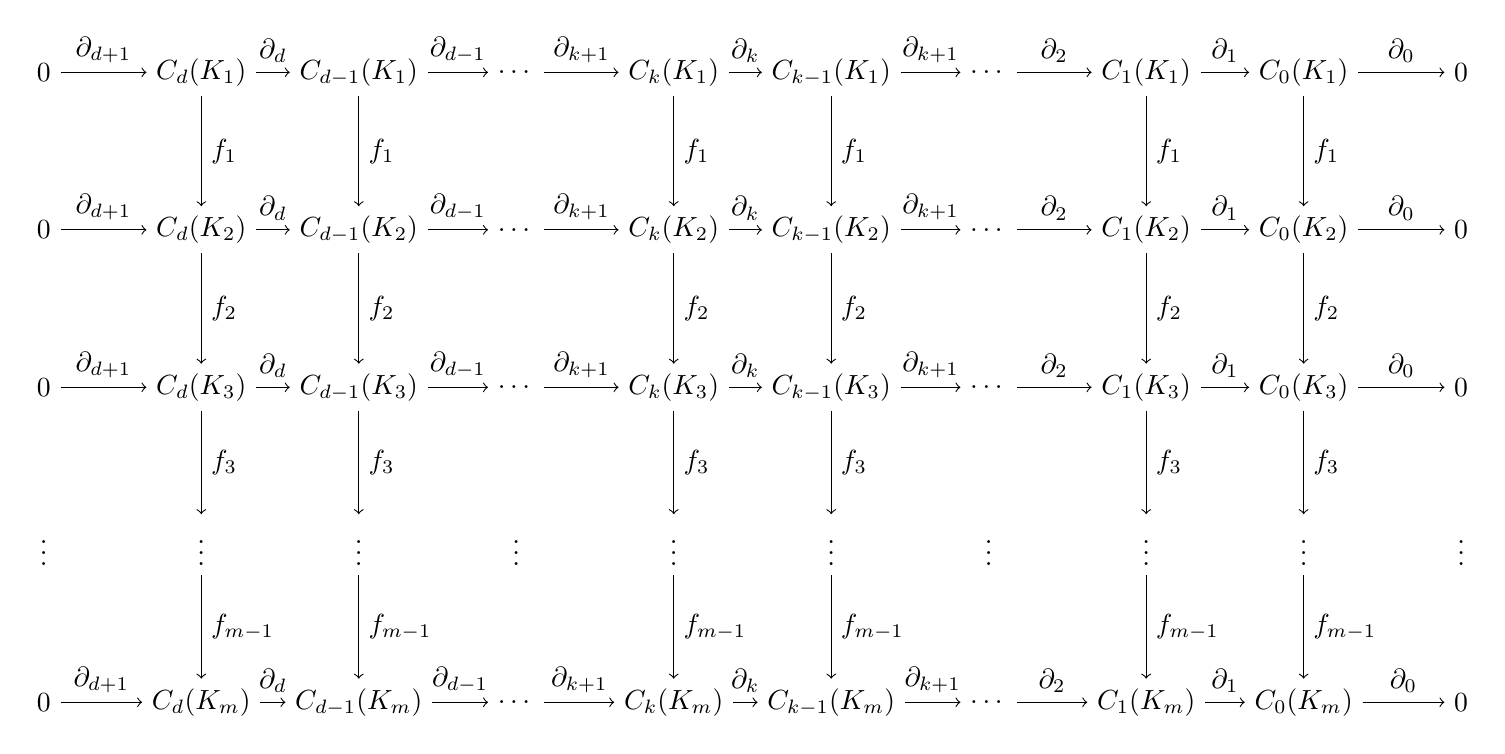
\begin{tikzpicture}[node distance=2cm, auto]
	% Define nodes
	\node (01) {$0$};
	\node (cdk1) [right of=01] {$C_d(K_1)$};
	\node (cd1k1) [right of=cdk1] {$C_{d-1}(K_1)$};
	\node (cd2k1) [right of=cd1k1] {$\dots$};
	\node (ckk1) [right of=cd2k1] {$C_k(K_1)$};
	\node (ck1k1) [right of=ckk1] {$C_{k-1}(K_1)$};
	\node (ck2k1) [right of=ck1k1] {$\dots$};
	\node (c1k1) [right of=ck2k1] {$C_1(K_1)$};
	\node (c0k1) [right of=c1k1] {$C_0(K_1)$};
	\node (012) [right of=c0k1] {$0$};

	\node (02) [below of=01] {$0$};
	\node (cdk2) [right of=02] {$C_d(K_2)$};
	\node (cd1k2) [right of=cdk2] {$C_{d-1}(K_2)$};
	\node (cd2k2) [right of=cd1k2] {$\dots$};
	\node (ckk2) [right of=cd2k2] {$C_k(K_2)$};
	\node (ck1k2) [right of=ckk2] {$C_{k-1}(K_2)$};
	\node (ck2k2) [right of=ck1k2] {$\dots$};
	\node (c1k2) [right of=ck2k2] {$C_1(K_2)$};
	\node (c0k2) [right of=c1k2] {$C_0(K_2)$};
	\node (022) [right of=c0k2] {$0$};

	\node (03) [below of=02] {$0$};
	\node (cdk3) [right of=03] {$C_d(K_3)$};
	\node (cd1k3) [right of=cdk3] {$C_{d-1}(K_3)$};
	\node (cd2k3) [right of=cd1k3] {$\dots$};
	\node (ckk3) [right of=cd2k3] {$C_k(K_3)$};
	\node (ck1k3) [right of=ckk3] {$C_{k-1}(K_3)$};
	\node (ck2k3) [right of=ck1k3] {$\dots$};
	\node (c1k3) [right of=ck2k3] {$C_1(K_3)$};
	\node (c0k3) [right of=c1k3] {$C_0(K_3)$};
	\node (032) [right of=c0k3] {$0$};

	\node (00) [below of=03] {$\vdots$};
	\node (cdk0) [right of=00] {$\vdots$};
	\node (cd1k0) [right of=cdk0] {$\vdots$};
	\node (cd2k0) [right of=cd1k0] {$\vdots$};
	\node (ckk0) [right of=cd2k0] {$\vdots$};
	\node (ck1k0) [right of=ckk0] {$\vdots$};
	\node (ck2k0) [right of=ck1k0] {$\vdots$};
	\node (c1k0) [right of=ck2k0] {$\vdots$};
	\node (c0k0) [right of=c1k0] {$\vdots$};
	\node (000) [right of=c0k0] {$\vdots$};
	
	\node (0m) [below of=00] {$0$};
	\node (cdkm) [right of=0m] {$C_d(K_m)$};
	\node (cd1km) [right of=cdkm] {$C_{d-1}(K_m)$};
	\node (cd2km) [right of=cd1km] {$\dots$};
	\node (ckkm) [right of=cd2km] {$C_k(K_m)$};
	\node (ck1km) [right of=ckkm] {$C_{k-1}(K_m)$};
	\node (ck2km) [right of=ck1km] {$\dots$};
	\node (c1km) [right of=ck2km] {$C_1(K_m)$};
	\node (c0km) [right of=c1km] {$C_0(K_m)$};
	\node (0m2) [right of=c0km] {$0$};


	% Draw edges
	\path[->]
	(01) edge node {$\partial_{d+1}$} (cdk1)
	(cdk1) edge node {$\partial_d$} (cd1k1)
	(cd1k1) edge node {$\partial_{d-1}$} (cd2k1)
	(cd2k1) edge node {$\partial_{k+1}$} (ckk1)
	(ckk1) edge node {$\partial_k$} (ck1k1)
	(ck1k1) edge node {$\partial_{k+1}$} (ck2k1)
	(ck2k1) edge node {$\partial_2$} (c1k1)
	(c1k1) edge node {$\partial_1$} (c0k1)
	(c0k1) edge node {$\partial_0$} (012)

	(02) edge node {$\partial_{d+1}$} (cdk2)
	(cdk2) edge node {$\partial_d$} (cd1k2)
	(cd1k2) edge node {$\partial_{d-1}$} (cd2k2)
	(cd2k2) edge node {$\partial_{k+1}$} (ckk2)
	(ckk2) edge node {$\partial_k$} (ck1k2)
	(ck1k2) edge node {$\partial_{k+1}$} (ck2k2)
	(ck2k2) edge node {$\partial_2$} (c1k2)
	(c1k2) edge node {$\partial_1$} (c0k2)
	(c0k2) edge node {$\partial_0$} (022)
	
	(03) edge node {$\partial_{d+1}$} (cdk3)
	(cdk3) edge node {$\partial_d$} (cd1k3)
	(cd1k3) edge node {$\partial_{d-1}$} (cd2k3)
	(cd2k3) edge node {$\partial_{k+1}$} (ckk3)
	(ckk3) edge node {$\partial_k$} (ck1k3)
	(ck1k3) edge node {$\partial_{k+1}$} (ck2k3)
	(ck2k3) edge node {$\partial_2$} (c1k3)
	(c1k3) edge node {$\partial_1$} (c0k3)
	(c0k3) edge node {$\partial_0$} (032)

	(0m) edge node {$\partial_{d+1}$} (cdkm)
	(cdkm) edge node {$\partial_d$} (cd1km)
	(cd1km) edge node {$\partial_{d-1}$} (cd2km)
	(cd2km) edge node {$\partial_{k+1}$} (ckkm)
	(ckkm) edge node {$\partial_k$} (ck1km)
	(ck1km) edge node {$\partial_{k+1}$} (ck2km)
	(ck2km) edge node {$\partial_2$} (c1km)
	(c1km) edge node {$\partial_1$} (c0km)
	(c0km) edge node {$\partial_0$} (0m2)

	(cdk1) edge node {$f_1$} (cdk2)
	(cdk2) edge node {$f_2$} (cdk3)
	(cdk3) edge node {$f_3$} (cdk0)
	(cdk0) edge node {$f_{m-1}$} (cdkm)

	(cd1k1) edge node {$f_1$} (cd1k2)
	(cd1k2) edge node {$f_2$} (cd1k3)
	(cd1k3) edge node {$f_3$} (cd1k0)
	(cd1k0) edge node {$f_{m-1}$} (cd1km)

	(ckk1) edge node {$f_1$} (ckk2)
	(ckk2) edge node {$f_2$} (ckk3)
	(ckk3) edge node {$f_3$} (ckk0)
	(ckk0) edge node {$f_{m-1}$} (ckkm)

	(ck1k1) edge node {$f_1$} (ck1k2)
	(ck1k2) edge node {$f_2$} (ck1k3)
	(ck1k3) edge node {$f_3$} (ck1k0)
	(ck1k0) edge node {$f_{m-1}$} (ck1km)

	(c1k1) edge node {$f_1$} (c1k2)
	(c1k2) edge node {$f_2$} (c1k3)
	(c1k3) edge node {$f_3$} (c1k0)
	(c1k0) edge node {$f_{m-1}$} (c1km)

	(c0k1) edge node {$f_1$} (c0k2)
	(c0k2) edge node {$f_2$} (c0k3)
	(c0k3) edge node {$f_3$} (c0k0)
	(c0k0) edge node {$f_{m-1}$} (c0km);
\end{tikzpicture}
}


\section*{Overview of Problem and Methodology}

\begin{itemize}
	\item focus on binary classification
	\item ``we seek to classify teo different probability distributions supported on teo disjoint manifolds $M_a, M_b \subset \R^d$''
	\item take $T \subset M_a \cup M_b = M$ uniformly and densely 
	\item train the NN $\nu : \R^d \to [0, 1]$ on $T$ until well-trained
	\item deliberately choose $M_a$ and $M_b$ to have topologically complicated decision boundary $D \subset \R^d$
	\item results will show that a well-trained NN reduces the topology on a layer-by-layer basis until $D$ is a hyperplane in $\R^p$ in the last layer
	\item In our approach, we can only indirectly observe $\nu_j(D)$ using $\nu_j(M_a), \nu_k(M_b)$, but not directly, i.e. no explicit $\omega(D)$
\end{itemize}


\section*{Real Versus Simulated Data}

\begin{itemize}
	\item In short, we use both real and simulated data
	\item Simulated Data:
		\begin{itemize}
			\item Has well-defined topological features that are known before-hand
			\item Clean samples, so we can skip denoising (step (i))
			\item Samples uniformly distributed on $M$
			\item Can always simulate data with a perfect classifier
		\end{itemize}
	\item Real-World Data:
		\begin{itemize}
			\item can have vastly more complicated topologies that are nearly impossible to determine
			\item may not have complete separation of categories, making it impossible to detangle
		\end{itemize}
	\item Simulated data allow us to pick the right $\varepsilon_*$ so we only need to compute homology at a single scale, whereas with real data we need to compute homology for a range of scales, making real data more computationally expensive
	\item In short, simulated data is easy, readily accessible, and non-trivial enough for this paper
	\item Hence, we do most of our experiments on simulated data and use some real world data at the end to validate the results from the simulation
\end{itemize}


\section*{Methodology}

\begin{itemize}
	\item 3 simulated data sets
	\item many, many NNs trained to the prescribed conditions
	\item Steps for computing $k_*$ and $\varepsilon_*$:
		\begin{enumerate}
			\item[(i)] Let $\varepsilon = 1$
			\item[(ii)] Choose $k_*$ so that $\beta_0(\VR_{k_*, 1}(X)) = \beta_0(M)$
			\item[(iii)] Let $k = k_*$
			\item[(iv)] Choose $\varepsilon_*$ so that $\beta_k(\VR_{k_*, 1}(X)) = \beta_k(M)$ for all $k \in \{1, 2, \dots, d-1\}$
		\end{enumerate}
	\item Key take away: Homology computations are way more expensive than training to near zero generalization error and can take up to 80 minutes for a single pair $(k_*, \varepsilon_*)$
\end{itemize}


\section*{Results and Discussions}
\begin{itemize}
	\item Topology changes and is simplified layer-by-layer
	\item Non-homeomorphic mappings (ReLU) reduce topology faster than homeomorphic mappinga (tahn)
	\item tanh struggles to change topology/requires more effort
	\item Network width does not generally have a significant effect on topological changes, but very narrow networks are much harder to train to a high accuracy
	\item Reducing network depth forces topological changes to concentrate in final layers rather than being evenly distributed. Network must be of sufficient length to change topology based on complexity of original data set
\end{itemize}


\section*{Consistency with Real-World Data}

\begin{itemize}
	\item Results from simulated experiments tested on 4 real-world data sets
	\item All experiments confirmed the same results that neural networks reduce topological complexities in our data and that non-homeomorphic mappings reduce topology faster than homeomoprhic mappings
\end{itemize}


\section*{Conclusion}

\begin{itemize}
	\item Restatement of results
	\item We concluded that ReLU changes topology faster than homeomorphic mappings, btu did not investigate the explicit mechanisms of how ReLU changes topology. We speculate that while affine mappings allow for translations, reflections, and contractions, composition with ReLU add the ability to fold space
\end{itemize}


\subsection*{Planning}
\begin{itemize}
	\item Visualization: write a Python script to visualize a data set over an underlying manifold and allow the user to select an $\epsilon$ value for the Vietoris-Rips complex. Should have a 3d visual. 
\end{itemize}


\end{document}



